% !TEX root = ./Thesis.tex

\section{Quantum description of NMR}

In this chapter, I will introduce the the quantum description of NMR. Including how
we use operators and superoperators to understand how states change under different conditons and how the energies of the system can be extracted.

\subsection{Nuclear Spin}

Nuclear spin can be treated as a type of angular momentum. Denoted by $\hat{I}$
it is comprised of a magnitude, $\lvert\hat{I}\rvert$, and a direction, $m_I$.
The magnitude is given by
\begin{equation}
  \lvert\hat{I}\rvert = \hbar\sqrt{I(I+1)}
\end{equation}
where $\hbar$ is the reduced Planck constant. The projection of $\hat{I}$ in
the $z$ direction, $\hat{I}_{z}$, is given by
\begin{equation}
  \hat{I}_{z} = m_I\hbar
\end{equation}
$m_{I}$ can take integer values from $-I$ to $+I$ shown in FIGprojection

For the commonly occuring case of a spin-1/2 nucleus, $I=1/2$ and $m_I = ±1/2$ and if we were to measure $\hat{I}_z$ we would get a value of $±1/2\hbar$ with an associated probability depending which state the system is in.

\begin{figure}
  \begin{center}
  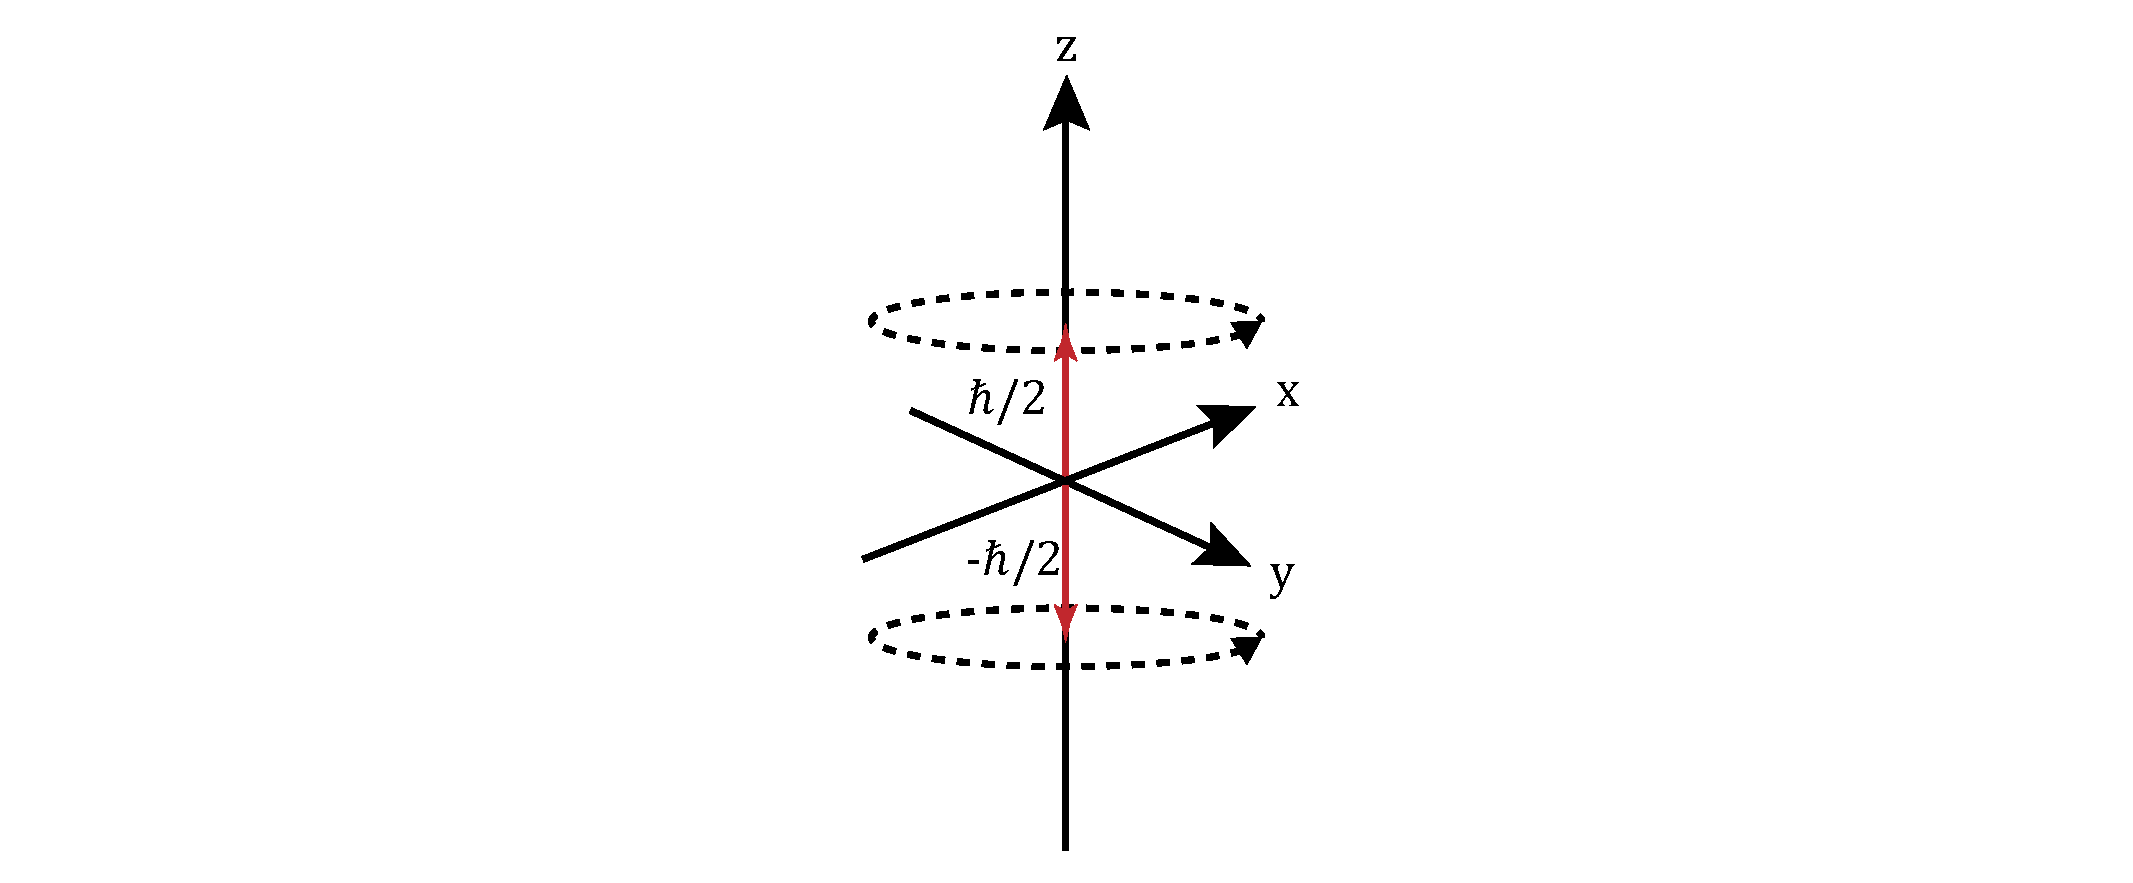
\includegraphics[textwidth=\textwidth,height=5cm,keepaspectratio]{StateProjection.pdf}
  \end{center}
  \caption{The projection of two states in a spin 1/2 nucleus (red arrow) with the magnitudes indicated (black arrow)}
  \label{fig:Projection}
\end{figure}

\subsection{Spin States}

If our spin-1/2 nucleus is placed in a magnetic field (taken to be oriented along $z$) it can exist in two states.
State one has $I = 1/2$, $m_I = 1/2$ and State two has $I = 1/2$, $m_I = -1/2$. We denote these as $\ket{I,m_I}$, this is called a 'ket', for simplicity we omit the $I$ and are left with
$\ket{m_I}$ and for spin-1/2 we call the two states $\ket{\alpha}$ or 'spin up' and $\ket{\beta}$ 'spin down.

$\ket{\alpha}$ and $\ket{\beta}$ are called the zeeman basis states and take the form

\begin{equation}
  \ket{\alpha} = \begin{pmatrix}
    1\\
    0
\end{pmatrix}
 \ket{\beta} = \begin{pmatrix}
   0\\
   1
\end{pmatrix}
\end{equation}

'bras' are also defined by taking the conjugate transpose of the ket, $\ket{\alpha}^{\dagger} =
\bra{\alpha}$ such that
\begin{equation}
  \bra{\alpha} = \begin{pmatrix}
    1 & 0
\end{pmatrix}
  \bra{\beta} = \begin{pmatrix}
  1 & 0
\end{pmatrix}
\end{equation}

The state, $\ket{\psi}$, of a two level system can now be completely decribed in this basis
as the linear combination of the basis states:
\begin{equation}\label{eqn:zeeman}
  \ket{\psi} = c_1\ket{\alpha} + c_2\ket{\beta} = \begin{pmatrix}
    c_1\\
    c_2
\end{pmatrix}
\end{equation}
\begin{equation}
  \bra{\psi} = c_1^*\bra{\alpha} + c_2^*\ket{\beta} = \begin{pmatrix}
    c_1^* & c_2^*
\end{pmatrix}
\end{equation}

These are normalised such that $c_1^2 + c_2^2 = 1$.

To complete the picture the sates must me orthonormal. Orthonormality between states exists if
if the inner product of the basis states $\ket{r_i} ~\text{and}~ \ket{r_j}$ satisifies the following conditions:

\begin{equation}
  \langle r_i\vert r_j\rangle = \delta_{ij}
\end{equation}

where the Kronecker delta is:
\begin{equation}
  \delta_{ij} = \begin{cases}
    0 & ~\text{if}~ i \ne j\\
    1 & ~\text{if}~ i = j
                \end{cases}
\end{equation}

where $\langle r_i\vert r_j\rangle = \delta_{ij}$ denotes taking the dot product between the two
vectors $\ket{r_i}$ and $\ket{r_j}$.

The outer product of the basis state, $\ket{r_n}$, for an N-spin system must satisfy:
\begin{equation}
  \sum_{n=1}^{N} \ket{r_n}\bra{r_n} = \mathbb{1}
\end{equation}

where $\mathbb{1}$ is an N by N identity matrix.

The inner product is used to quantifuy the projeciton of one state along another. Take our example from \ref{eqn:zeeman}, we can construct inner products and determine the projection
of $\ket{\psi}$ on $\ket{\alpha}$ and $\ket{\beta}$.
\begin{equation}
  \langle\alpha\vert\psi\rangle = c_1 & \langle\beta\vert\psi\rangle = c_2
\end{equation}

When a second spin is introduced, the Hilbert space is extended to accommodate additional spin
states by taking the tensor product of the basis states


\begin{align}
\ket{\alpha_{1}\alpha_{2}} = \ket{\alpha_1} \otimes \ket{\alpha_2} = \begin{pmatrix}
  1\\
  0\\
  0\\
  0
\end{pmatrix} &
\ket{\alpha_{1}\beta_{2}} = \ket{\alpha_1} \otimes \ket{\beta_2} = \begin{pmatrix}
  0\\
  1\\
  0\\
  0
\end{pmatrix}\\
\ket{\beta_{1}\alpha_{2}} = \ket{\beta_1} \otimes \ket{\alpha_2} = \begin{pmatrix}
  0\\
  0\\
  1\\
  0
\end{pmatrix} &
\ket{\beta_{1}\beta_{2}} = \ket{\beta_1} \otimes \ket{\beta_2} = \begin{pmatrix}
  0\\
  0\\
  0\\
  1
\end{pmatrix}
\end{align}
The subscripts indicate which spin we are reffering to, e.g. $\ket{\beta_1\alpha_2}$ means that
spin 1 is in the $\beta$ state and spin 2 is in the $\alpha$ state.

To summarize, we can use bras and kets to describe the spin state of an N-spin system using the Zeeman basis states. We will now at manipulating these staes with operators.

\subsection{Operators}

Operators act on states. To explain this, let's consider a generic operator $\hat{B}$ with eigenstates $\ket{\alpha}$ and $\ket{beta}$. When a state is acted upon by an operator it is denoted by:
\begin{equation}
  \hat{B}\ket{\alpha} = b\ket{\alpha}
\end{equation}

the same state is returned, multiplied by some scalar $b$, that is an eigenvalue of $\ket{\alpha}$
in the operator basis B.

The expectation value of an operator can be found by:
\begin{equation}\label{eqn:expectation}
  \langle\hat{B}\rangle = \langle\alpha\vert\hat{B}\vert\alpha\rangle = b\langle\alpha\vert\alpha\rangle = b
\end{equation}

this returns the eigenvalue.

In NMR there are three angular momentum operators $\hat{I}_x$, $\hat{I}_y$ and $\hat{I}_z$. These are defined by the Pauli matrices multiplied by $\frac{\hbar}{2}$.

\begin{equation}
  \hat{I}_x=\frac{\hbar}{2}\begin{pmatrix}
    0 & 1\\
    1 & 0
\end{pmatrix}
\hat{I}_y=\frac{\hbar}{2i}\begin{pmatrix}
  0 & 1\\
  -1 & 0
\end{pmatrix}
\hat{I}_z=\frac{\hbar}{2}\begin{pmatrix}
  1 & 0\\
  0 & 1
\end{pmatrix}
\end{equation}

as an example, let's take the example from before of a spin-1/2 particle in a magnetic field
and see what happens if we were to project the $\ket{\alpha}$ state along the z-axis.
\begin{equation}\label{eqn:operators}
  \hat{I}_x\ket{\alpha} = \frac{\hbar}{2}\begin{pmatrix}
    0 & 1\\
    1 & 0
\end{pmatrix}
\begin{pmatrix}
  1\\
  0
\end{pmatrix} = \frac{\hbar}{2}\begin{pmatrix}
  1\\
  0
\end{pmatrix} = \frac{\hbar}{2}\ket{\alpha}
\end{equation}
We find that $\frac{\hbar}{2}$ is the eigenvalue of $\ket{\alpha}$ for the operator $\hat{I}_z$. For ease of handling in the following examples we will take $\hbar$ = 1.

We will now examine three more operators and explore how they act on states. They are the total square angular momentum, $\hat{I}^2$ and the two shift operators $\hat{I}^+$ and $\hat{I}^-$ defined as the following:

\begin{align}
  \hat{I}^2 =& \hat{I}_x^2 + \hat{I}_y^2 + \hat{I}_z^2\\
  \hat{I}^+ =& \hat{I}_x + i\hat{I}_y\\
  \hat{I}^- =& \hat{I}_x - i\hat{I}_y
\end{align}
They act on states according to:
\begin{align}
  \hat{I}^2\ket{I,m_I} =& I(I+1)\ket{I, m_I}\\
  \hat{I}^+\ket{I,m_I} =& \sqrt{(I(I+1)-m_I(m_I+1))}\ket{I,m_{I+1}}\\
  \hat{I}^-\ket{I,m_I} =& \sqrt{(I(I+1)-m_I(m_I-1))}\ket{I,m_{I-1}}
\end{align}
Using our spin-1/2 particle in a magnetic field as an example we'll let these operators act on the $\ket{\alpha}$ state
\begin{align}
  \hat{I}^2\ket{\alpha} =& \frac{3}{4}\ket{\alpha}\\
  \hat{I}^+\ket{\alpha} =& 0\\
  \hat{I}^-\ket{\alpha} =& {\beta}
\end{align}

We can see if two operators commute by using the commutator which is defined as:
\begin{equation}
  [\hat{A},\hat{B}] = \hat{A}\hat{B} - \hat{B}\hat{A}
\end{equation}

If $[\hat{A},\hat{B}] = 0$ the operators are said to commute. The $\hat{I}_z$, $\hat{I}_z$ and $\hat{I}_z$
have what is called cyclic commutation rules:
\begin{align}\label{eqn:commutator}
  [\hat{I}_x,\hat{I}_y] = i\hat{I}_z\\
  [\hat{I}_y,\hat{I}_z] = i\hat{I}_x\\
  [\hat{I}_x,\hat{I}_z] = i\hat{I}_y
\end{align}

These relationships are important in NMR as they help govern the rules for the rotations of spins.

\subsection{Superoperators}

Like states, that can be transformed by operators, operators can be transformed by the imaginitively
named 'superoperators' these are denoted by a double hat.

To start, let's take a simple commutation superoperator, $\hat{\hat{A}}$, defined as:
\begin{equation}
  \hat{\hat{A}}\hat{B} = [\hat{A},\hat{B}] = \hat{A}\hat{B} - \hat{B}\hat{A}
\end{equation}
Applying it to operator $\hat{B}$ results in the commutation of $\hat{A}$ and $\hat{B}$

In NMR, three rotational superoperators can be defined using the commutation superoperators from \ref{eqn:operators}:
\begin{equation}
 \hat{\hat{R}}_x(\theta) = \text{exp}\{-i\hat{\hat{I}}_x\theta\}\quad\hat{\hat{R}}_y(\theta) = \text{exp}\{-i\hat{\hat{I}}_y\theta\}\quad\hat{\hat{R}}_z(\theta) = \text{exp}\{-i\hat{\hat{I}}_z\theta\}
\end{equation}

These are applied to to the angular momentum operators using the sandwich formula:
\begin{equation}
  \hat{\hat{R}}_x(\theta)\hat{I}_z = \text{exp}\{-i\hat{\hat{I}}_x\theta\}\hat{I}_z\text{exp}\{+i\hat{\hat{I}}_x\theta\}
\end{equation}

The result of this is a rotation of $\hat{I}_z$ around the $x$-axis by an angle $\theta$:
\begin{equation}
  \hat{\hat{R}}_x(\theta)\hat{I}_z = \cos{\theta}\hat{I}_z - \sin{\theta}\hat{I}_y
\end{equation}

The rotational direction (sign of the $\sin{\theta}$ term) is determined by the right hand co-ordinate system defined in \ref{eqn:commutator}.

We will now discuss how these are used in describing the spin dynamics of a spin system.

\subsection{Density Operator}

The density operator gives us information on the state of groups of spins in a spin system. It is
vital to be able to spins in groups as the number of individual spins in a typical NMR experiment is
usually $>>10^20$.

Let's go back once again to a spin-1/2 particle in a magnetic field. Where $\ket{\psi}$ is some superposition state in the two level system such that:
\begin{align}
\ket{\psi} =& \begin{pmatrix}
    c_1\\
    c_2
\end{pmatrix} = c_1\ket{\alpha} + c_2\ket{\beta}\\
\bra{\psi} =& \begin{pmatrix}
  c_1^* & c_2^*
\end{pmatrix} = c_1^*\bra{\alpha} + c_2^*\bra{\beta}
\end{align}

The density operator has the form:
\begin{equation}
  \hat\rho = \ket{\psi}\bra{\psi} = \begin{pmatrix}
    c_1c_1^* & c_1c_2^*\\
    c_2c_1^* & c_2c_2^*
\end{pmatrix}
\end{equation}

If the number of spins is increased, the denstiy operator's form does not change instead it provides
an average fo the entire group of spin states. The population of a given state is given by the expectation value of the density operator as in \ref{eqn:expectation}. If we would like to know
the population of state $\ket{\alpha}$ we would perform the following:
\begin{equation}
  \langle\alpha\vert\hat\rho\vert\alpha\rangle = \langle\alpha\vert\psi\rangle \langle\alpha\vert\psi\rangle = c_1^*c_1
\end{equation}

The diagonal elements of $\hat\rho$ are state populations.

The off-diagonal elements are coherences between states. These coherences are complex numbers and two coherences between the same pair of states are complex cojugates of each other. e.g.:
\begin{equation}
  \langle\alpha\vert\hat\rho\vert\beta\rangle = (\langle\beta\vert\hat\rho\vert\alpha\rangle)^* = c_1c_2^* = (c_1^*c_2)^*
\end{equation}
The coherence order between two states in a magnetic field is defined as the difference in angular
momentum projection along the $z$ axis. In our two spin this would be(with $\hbar = 1$):
\begin{align}
  \hat{I}_z\ket{\beta} = m_\alpha = +\frac{1}{2}\ket{\alpha}\\
  \hat{I}_z\ket{\beta} = m_\beta = -\frac{1}{2}\ket{\beta}
\end{align}
We can use these results to calculate the coherence order of the coherence $\langle\alpha\vert\hat\rho\vert\beta\rangle$:
\begin{equation}
 m_\alpha - m_\beta = +1
\end{equation}
and conversely the coherence order of $\langle\beta\vert\hat\rho\vert\alpha\rangle$ is:
\begin{equation}
  m_\beta - m_\alpha = -1
\end{equation}

Now let's look at how $\hat\rho$ relates to the angular momentum operators give in \ref{eqn:operators}.

Usually in NMR there is only a small population difference between $\alpha$ and $\beta$, see \ref{Population}
but for this example let's imagine we have found a sufficiently strong enough field for a population difference of $0.1$. The density operator in this case would be:
\begin{equation}
  \hat\rho = \frac{1}{2}\begin{pmatrix}
    1 + 0.1 & 0\\
    0 & 1-0.1
\end{pmatrix}
\end{equation}
using the definition given in \ref{eqn:operators} we can re-write this as
\begin{equation}
  \hat\rho = \frac{1}{2}\hat{\mathbb{1}} + 0.1\hat{I}_z
\end{equation}
$\hat{\mathbb{1}}$ is identity matrix and corresponds to no population difference between $\ket{\alpha}$ and $\ket{\beta}$.

$\hat{\mathbb{1}}$ is unaffected by rotations so can be ignored in the context of NMR
and so we write
\begin{equation}
  \hat{\rho} = 0.1\hat{I}_z
\end{equation}
to describe the $z$ magnetisation of our sample.

The density operator can also be used to to describe the evolution of a spin system under operations. If we applied a $90$ degree pulse along the $y$ axis, denoted using radians by $(\pi/2)_y$. That is the equivalent of propagating the initial density operator, $\rho_0$
under the rotation superoperator $\hat{\hat{R}}_y(\pi/2)$:
\begin{equation}
  \hat{\rho}_1 = \hat{\hat{R}}_y(\frac{\pi}{2})\hat\rho_0 = \text{exp}\{-i(\frac{\pi}{2})\hat{\hat{I}}_y\}\hat{I}_z\text{exp}\{+i(\frac{\pi}{2})\hat{\hat{I}}_y\} = \hat{I}_x
\end{equation}
Now the magnetisation is in the $x$-axis it will begin to precess about the $z$-axis which using our notation is the equivalent of of propagating $\hat{I}_x$ ($\hat{\rho}_1$)
under $\hat{\hat{R}}_z(\omega t)$:
\begin{align}\label{eqn:propagate}
  \hat{\rho}_2 = \hat{\hat{R}}_z(\omega t)\hat{\rho}_1 =& \text{exp}\{-i\omega t\hat{\hat{I}}_z\}\hat{I}_x\text(exp)\{+i\omega t\hat{\hat{I}}_z\}\\
   =& \cos(\omega t)\hat{I}_x + \sin(\omega t)\hat{I}_y
\end{align}
where $\omega$ is the larmour frequency, and $t$ is time.

the $\text{exp}\{i\omega t\}$ is called a propagator, because it propagates the density operator in time.

The Hamiltonian, the energy operator, describes how the system evolves in time and uses progators, rotational superoperators and the density operator in order to do so.

\subsection{The Hamiltonian}

As mentioned the Hamiltonian is the energy operator. It provides information on the enrgies of states in a system.

If we let $\ket{\psi_1}$ and $\ket{\psi_2}$ be eigenstates of the Hamiltonian $\hat{H}$ then
\begin{align}
  \hat{H}\ket{\psi_1} = E_1\ket{\psi_1}\\
  \hat{H}\ket{\psi_2} = E_2\ket{\psi_2}
\end{align}

The Hamiltonian can also be expressed in matrix form:
\begin{equation}
  \hat{H} = \begin{pmatrix}
    E_1 & 0\\
    0 & E_2
\end{pmatrix}
\end{equation}
If the Hamiltonian is written in the eigenbasis of the system its main diagonal correspond to state energies and it has values of $0$ everywhere else.

The evolution in time of a quantum system is described by the Schr\"odinger equation:
\begin{equation}
  i\hbar\frac{\partial}{\partial{t}}\ket{\psi} = \hat{H}\ket{\psi}
\end{equation}
The $\hbar$ was included for completeness sake and will again be set to equal $1$.

In NMR we describe the dynamics of a system using the density operator evolution rather than the evolution of the states using
\begin{align}
  \frac{\partial}{\partial{t}}\ket{\psi} = -i\hat{H}\ket{\psi}\\
  \frac{\partial}{\partial{t}}\bra{\psi} = i\hat{H}\bra{\psi}
\end{align}

we can derive\citep{Neumann2018}:
\begin{align}
  \frac{\partial}{\partial{t}}\hat\rho\quad=&\quad \frac{\partial}{\partial{t}}[\ket{\psi}\bra{\psi}]\\
  =&\quad[\frac{\partial}{\partial{t}}\ket{\psi}]\bra{\psi} + \ket{\psi}[\frac{\partial}{\partial{t}}\bra{\psi}]\\
  =&\quad-i\hat{H}\ket{\psi}\bra{\psi} + i\ket{\psi}\bra{\psi}
\end{align}
to give the relationship
\begin{equation}
  \frac{\partial}{\partial{t}}\hat\rho = -i[\hat{H},\hat\rho]
\end{equation}
this is called the Louisville von Neumann equation.

Returning to our spin-1/2 particle in a magnetic field. The Hamiltonian is initially
proportional to the $z$ angular momentum operator
\begin{equation}
  \hat{H} = \omega\hat{I}_z
\end{equation}

where $\omega = -\gamma B_0$. In matrix form, in our original zeeman basis, the Hamiltonian is:
\begin{equation}
  \hat{H} = \begin{pmatrix}
+\frac{\omega}{2} & 0\\
0 & -\frac{\omega}{2}
\end{pmatrix}
\end{equation}
where
\begin{equation}
  \hat{H}\ket{\alpha} = +\frac{\omega}{2}\ket{\alpha}
\end{equation}

The density operator evolves under a Hamiltonian like so:
\begin{equation}
  \hat\rho(t) = \text{exp}\{-i\hat{H}t\}\hat\rho(0)\text{exp}\{+i\hat{H}t\}
\end{equation}

In \ref{eqn:propagate}, we saw that the precession of a spin-1/2 particle in a magnetic field can be described using the rotation superoperator around the $z$-axis $\hat{\hat{R}}_z(\omega t)$. We know that for this system its analagous to $\hat{H} = \omega\hat{I}_4$.

If the density operator commutes with the Hamiltonian there is no evolution of the system
this can be seen more clearly using propagators with $\hat{H} = \omega\hat{I}_z$ and $\rho(0) = \hat{I}_z$
\begin{equation}
  \rho(t) = \text{exp}\{-i\omega t\hat{\hat{I}}_z\}\hat{I}_z\text{exp}\{+i\omega t\hat{\hat{I}}_z\} = \hat{I}_z
\end{equation}
If the density operator does not commute with the Hamiltonian it will evolve. To demostrate this we use $\hat{H} = \omega\hat{I}_z$ as before  however this time $\hat\rho(0) = \hat{I}_x$
\begin{equation}
  \hat\rho(t) = \text{exp}\{-i\omega t\hat{\hat{I}}_z\}\hat{I}_x\text{exp}\{+i\omega t\hat{\hat{I}}_z\} = \cos(\omega t)\hat{I}_x + \sin(\omega t)\hat{I}_y
\end{equation}
The Hamiltonian for multi-spin system is slightly more complicated. Consider a two spin
system $I_1$ and $I_2$ with $J$-coupling $J_{12}$ the Hamiltonian then becomes:
\begin{equation}
  \hat{H} = \omega_1\hat{I}_1 + \omega_2\hat{I}_2 + 2\pi J_{12}\hat{\mathbf{I}}_1.\hat{\mathbf{I}}_2
\end{equation}
where $\hat{\mathbf{I}}_1.\hat{\mathbf{2}}_2 = \hat{I}_{1x}\hat{I}_{2x} + \hat{I}_{1y}\hat{I}_{2y} + \hat{I}_{1z}\hat{I}_{2z}$.
In matrix form in the zeeman basis this is:
\begin{equation}
  \hat{H} = \frac{1}{2}\begin{pmatrix}
    +\omega_1 + \omega_2 + \pi J_{12} & 0 & 0 & 0\\
    0 & +\omega_1 - \omega_2 - \pi J_{12} & 2\pi J_{12} & 0\\
    0 & 2\pi J_{12} & -\omega_1 + \omega_2 - \pi J_{12} & 0\\
    0 & 0 & 0 & -\omega_1 - \omega_2 - \pi J_{12}
\end{pmatrix}
\end{equation}

The zeeman basis is no longer an eigenbasis of the Hamiltonian because the $J$-coupling
introduces off-diagonal terms. In practice, when $|\omega_1-\omega_2| >> 2\pi J_{12}$
these terms are ignored because the zeeman basis is approxiamely the eigen basis of the Hamiltonian. This is termed the secular approxiamation.

However, when this is not the case, the Hamiltonian requires diagonalisation which is beyond the scope of this introduction but will be addressed if needed in later chapters.
